We observe that Dynamic Frontier (DF) Leiden outperforms both Naive-dynamic (ND) and Delta-screening (DS) Leiden, as shown in Section \ref{sec:performance-comparison}. Therefore, we focus most of our discussion below on how to extend the DF approach to the Leiden algorithm. The procedure to extend the ND and DS approaches to the Leiden algorithm are quite similar\ignore{, and are discussed at the end of this section}. Table \ref{tab:terminology} shows the terminology used in this report.




\subsection{No continued passes}
\label{sec:no-continued-passes}

A straightforward application of the DF approach to the Leiden algorithm involves processing incrementally identified affected vertices during the local-moving phase of the algorithm, refining the obtained communities in the subsequent phase, aggregating the refined communities into a super-vertex graph (where each refined community is collapsed into a super-vertex), and repeating this process until convergence is reached. However, for small batch updates, convergence may occur after just one pass of the algorithm, at which point the algorithm would terminate. This results in suboptimal communities with low modularity, as the communities generated from the refinement phase did not have the opportunity to hierarchically merge and form tightly-knit groups with dense internal connections and sparse inter-community links. An example of the communities returned in the absence of further processing is shown in Figure \ref{fig:subrefine-stages--01}, given a batch update. It is important to note that this issue does not arise in the absence of the refinement phase --- it occurs specifically when refinement is applied, as it forces the communities identified during the local-moving phase to be divided into smaller sub-communities. 

\begin{figure*}[hbtp]
  \centering
  \subfigure[No continued passes]{
    \label{fig:subrefine-stages--01}
    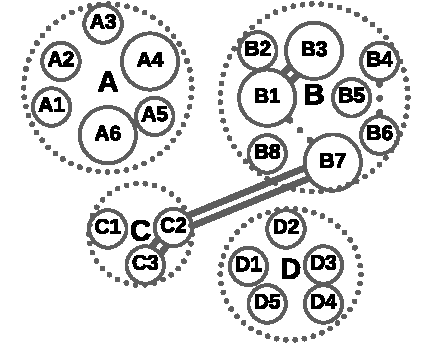
\includegraphics[width=0.31\linewidth]{out/subrefine-stages01.pdf}
  }
  \subfigure[Full Refine]{
    \label{fig:subrefine-stages--02}
    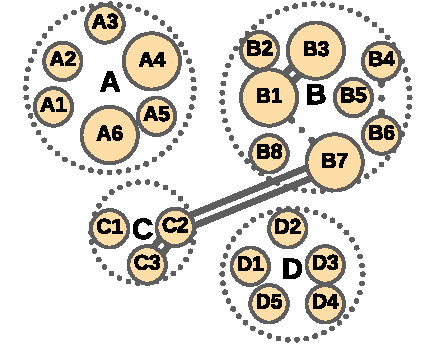
\includegraphics[width=0.31\linewidth]{out/subrefine-stages02.pdf}
  }
  \subfigure[Subset Refine]{
    \label{fig:subrefine-stages--03}
    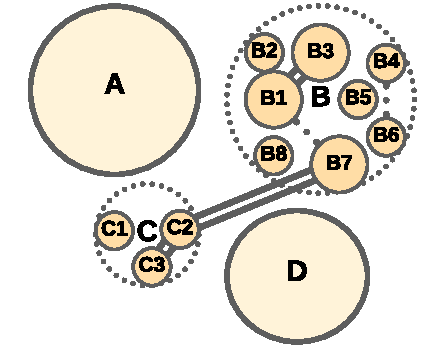
\includegraphics[width=0.31\linewidth]{out/subrefine-stages03.pdf}
  } \\[-1ex]
  \caption{Comparison of \textit{No continued passes}, \textit{Full Refine}, and \textit{Subset Refine} methods. Here, circles represent communities (or subcommunities post refinement), dotted circles denote old parent communities during the local-moving phase\ignore{community bounds}, dotted lines indicate edge deletions, double lines signify edge insertions, and a brown fill indicates mandated further processing. Pre-existing edges are not shown\ignore{for simplicity}. With \textit{No continued passes}, all communities are refined after the local-moving phase; however, it may converge prematurely with small batch updates, resulting in suboptimal community structures. The \textit{Full Refine} method processes all refined communities after they are aggregated into super-vertices. In contrast, with the \textit{Subset Refine} method, we selectively refine only a subset of communities based on the batch update, leaving the remaining communities unchanged.}
  \label{fig:subrefine-stages}
\end{figure*}





\subsection{Full Refine method}
\label{sec:full-refine-method}

Despite the above mentioned issues, we\ignore{still} aim to retain the refinement phase in the Leiden algorithm due to its beneficial properties, such as preventing the formation of poorly connected or even internally disconnected communities \cite{com-traag19}. To this end, unlike DF Louvain \cite{sahu2024shared}, we do not stop the algorithm after the first pass, but rather, run the algorithm until convergence occurs in a subsequent local-moving phase, where all vertices are processed, not just the affected ones. We refer to this method as \textbf{Full Refine}. Figure \ref{fig:subrefine-stages--02} shows an example of the communities returned with the \textit{Full Refine} method.




\subsection{Subset Refine method}
\label{sec:subset-refine-method}

Nevertheless, for small batch updates, only a few communities are typically affected, and only those need refinement. To identify these communities, we track vertices that migrate between communities during the local-moving phase and mark both their source and target communities as changed (i.e., needing refinement) because their sub-community structures may have been altered. However, the community membership IDs assigned to vertices during the local-moving phase can sometimes be inconsistent. For instance, a community labeled as $C = i$ might not contain a vertex with ID $i$ if that vertex has migrated to another community. This inconsistency can create problems during the refinement phase, where each vertex in the communities being refined must initially belong to its own community. To understand the issue, consider an example illustrated in Figure \ref{fig:subrefine-issue--1}. Here, say we selectively refine community $B$, which includes vertex $i$, but leave $C = i$ unchanged. In such a scenario, vertex $i$ may remain as an isolated sub-community disconnected from the rest of $C = i$. Worse, as shown in Figure \ref{fig:subrefine-issue--2}, vertices $j$ and $k$ could merge with vertex $i$ to form a sub-community $D = i$, resulting in two unconnected communities, $C = i$ and $D = i$, sharing the same ID. This issue arises only when refining a subset of communities and does not occur if all communities are refined. To address this, we must assign each community $C = i$ a new ID $i'$, where $i'$ corresponds to one of its constituent vertices. Additionally, we must update the total community edge weights and changed community flags to reflect the new community IDs, as these are initially tied to the old IDs.
% Legit operations due to a batch update

\begin{figure}[hbtp]
  \centering
  \subfigure[Disconnected isolated vertex]{
    \label{fig:subrefine-issue--1}
    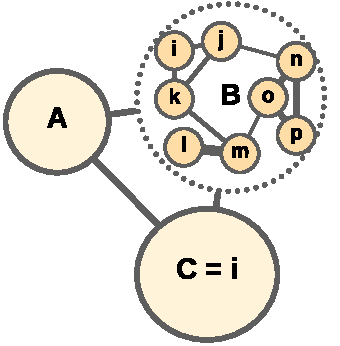
\includegraphics[width=0.45\linewidth]{out/subrefine-issue1.pdf}
  }
  \subfigure[Disconnected community formation]{
    \label{fig:subrefine-issue--2}
    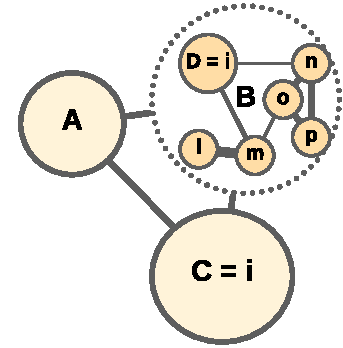
\includegraphics[width=0.45\linewidth]{out/subrefine-issue2.pdf}
  } \\[-1ex]
  \caption{Illustration of issues arising during the refinement phase when only a subset of communities is refined. Here, circles represent communities (or subcommunities after refinement), dotted circles indicate old parent communities (from the local-moving phase), and lines show both inter- and intra-community edges. Upon refinement of community $B$, subfigure (a) shows that vertex $i$ is isolated, but disconnected from community $C = i$, while subfigure (b) shows that further refinement forms sub-community $D = i$, which is disconnected from community $C = i$.}
  \label{fig:subrefine-issue}
\end{figure}
% Subfigure (a) demonstrates the isolation of vertex $i$ during selective refinement of community $B$, resulting in a disconnection from $C = i$. Subfigure (b) shows how further refinement can lead to the formation of two unconnected communities, $C = i$ and $D = i$, sharing the same ID. To resolve such inconsistencies, new IDs must be assigned to communities based on their constituent vertices, and associated data structures, including edge weights and flags, must be updated.


Next, we consider the impact of batch updates on the communities requiring refinement. Edge deletions within a community can cause it to split. However, if a community is isolated, the local-moving phase cannot find better community assignments for any of the vertices belonging to the community. In the extreme case, edge deletions within a community can also cause a community to be internally disconnected, if vertices within the community do not change their community assignments. This scenario can occur even if the community is not isolated. In order to address both concerns, refinement is the only way for such communities to split. Since community migrations do not occur, these communities would not be marked for refinement. Accordingly, for edge deletions in the batch update belonging to the same community, we mark the community as changed --- ensuring it is refined after the local-moving phase. Similarly, edge insertions affecting different parts of a community might also lead to a split, and must therefore be refined. Accordingly, for edge insertions in the batch update belonging to the same community, we mark the community as changed. Figure \ref{fig:community-split} shows an example of how these corner cases might occur with isolated communities, which may cause the community to split. We refer to this method of selective refinement of communities obtained from the local-moving phase of the algorithm, considering both vertex migration and the batch update, as \textbf{Subset Refine}. Figure \ref{fig:subrefine-stages--03} shows an example of the communities returned with the \textit{Subset Refine} method. Note that only a subset of the communities are processed into subcommunities.
% Edge deletions and insertions within a community may cause it to split. However, if the community is isolated, the local-moving phase will not be able to partition such communities --- since there are no better communities to move to, for any of the member vertices. In order to address this issue, such communities must be refined. Additionally, refining non-isolated communities with intra-community edge deletions and insertions facilitates splitting of such communities.

Note that selective refinement is applied only in the first pass of the Leiden algorithm, while all communities are refined in subsequent passes. This is because untouched communities are already aggregated into super-vertices during the first pass. In the later passes, tracking communities across the super-vertex hierarchy would be costly, and the time saved by selective refinement in these smaller graphs wouldn't justify the overhead.
% Note that selective refinement is performed only in the first pass of Leiden algorithm --- in the remaining passes, all the communities are refined. This is because further passes operate on super-vertex graphs, which are relatively small in size, and also because the tracking the communities across the hierarchy would be expensive, and time savings obtained due to selective refinement in super-vertex graphs would not be worth the overhead.

\begin{figure}[hbtp]
  \centering
  \subfigure{
    \label{fig:community-split--all}
    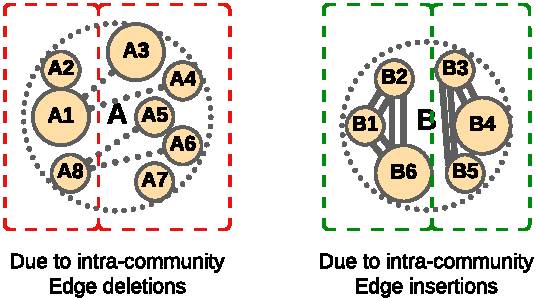
\includegraphics[width=0.80\linewidth]{out/community-split-all.pdf}
  } \\[-1ex]
  \caption{Demonstration of how decreasing or increasing edge density within a community can cause it to split. Here, circles show refined subcommunities, while dotted circles represent the original parent communities from the local-moving phase. Dotted lines indicate edge deletions, double lines represent edge insertions, and brown-filled areas mark regions needing further processing. Red and green boundaries highlight possible split points due to batch updates.}
  \label{fig:community-split}
\end{figure}





\subsection{Optimized Aggregation method}
\label{sec:optimized-aggregation-method}

However, the above selective refinement method hardly improves the performance of the DF Leiden, particularly for small batch updates. For these smaller updates, the aggregation phase remains a major bottleneck. This is mainly due to the selective refinement of communities, which results in a large difference in the sizes of communities to be aggregated --- the refined communities tend to be small, while the unrefined communities tend to be large. This creates a heavy workload for threads aggregating these unrefined communities into super-vertices. To ensure better load balancing, heavily loaded threads should be assigned minimal additional communities. Dynamic work scheduling can help, with each thread being assigned a smaller range of community IDs, or chunks. However, chunk sizes that are too small can introduce significant scheduling overhead. Through experimentation with chunk sizes from $1$ to $2048$ --- on large real-world graphs (given in Table \ref{tab:dataset-large}), with uniformly random batch updates consisting of $80\%$ edge insertions and $20\%$ edge deletions (see Section \ref{sec:batch-generation}), on batch sizes of $10^{-7}|E|$, $10^{-5}|E|$, and $10^{-7}|E|$, where $|E|$ is the number of edges in the original graph --- we find that a chunk size of $32$ provides the best overall performance for ND, DS, and DF Leiden; as shown in Figure \ref{fig:aggregation-adjust-chunksize}. We refer to this method as \textbf{Optimized Aggregation}. Figure \ref{fig:subrefine-optimize} illustrates the\ignore{mean} runtime of DF Leiden based on\ignore{the three methods mentioned,} \textit{Full Refine}, \textit{Subset Refine}, and \textit{Optimized Aggregation} methods, on large graphs with batch updates of size $10^{-7}|E|$ to $0.1|E|$.

\begin{figure}[!hbt]
  \centering
  \subfigure[Relative runtimes on uniformly random batch updates of size $10^{-7}|E|$]{
    \label{fig:aggregation-adjust-chunksize--batch7}
    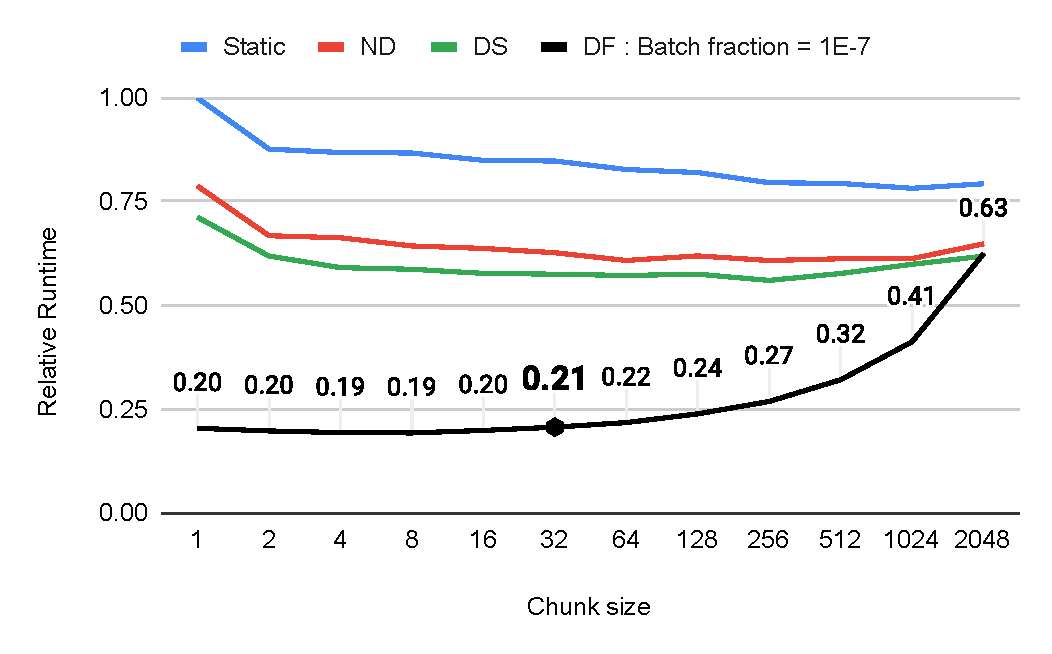
\includegraphics[width=0.98\linewidth]{out/aggregation-adjust-chunksize7.pdf}
  }
  \subfigure[Relative runtimes on uniformly random batch updates of size $10^{-5}|E|$]{
    \label{fig:aggregation-adjust-chunksize--batch5}
    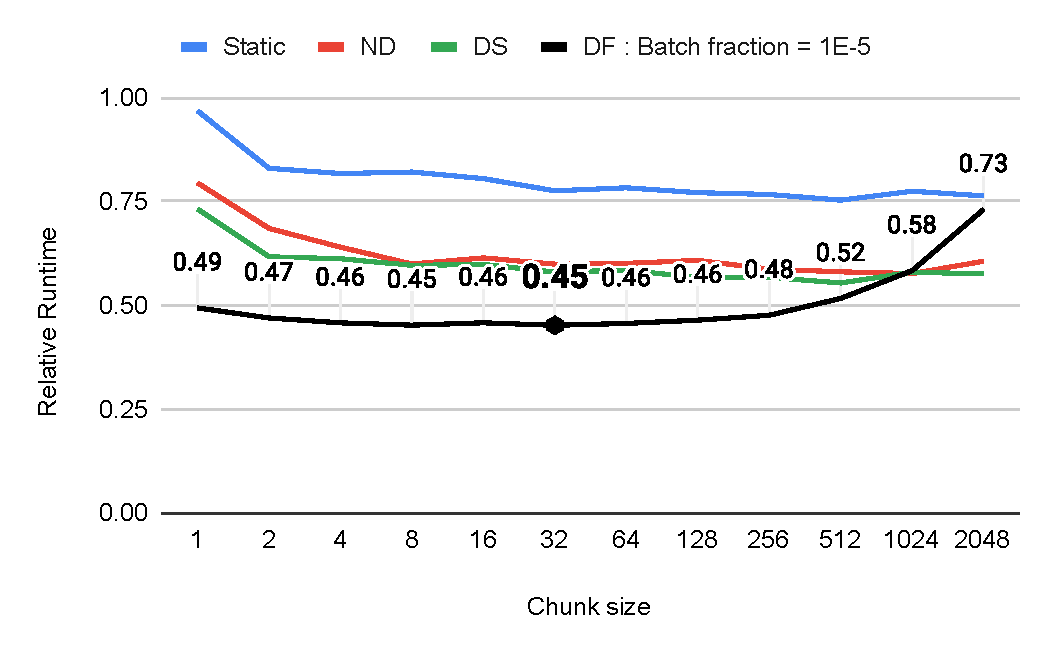
\includegraphics[width=0.98\linewidth]{out/aggregation-adjust-chunksize5.pdf}
  }
  \subfigure[Relative runtimes on uniformly random batch updates of size $10^{-3}|E|$]{
    \label{fig:aggregation-adjust-chunksize--batch3}
    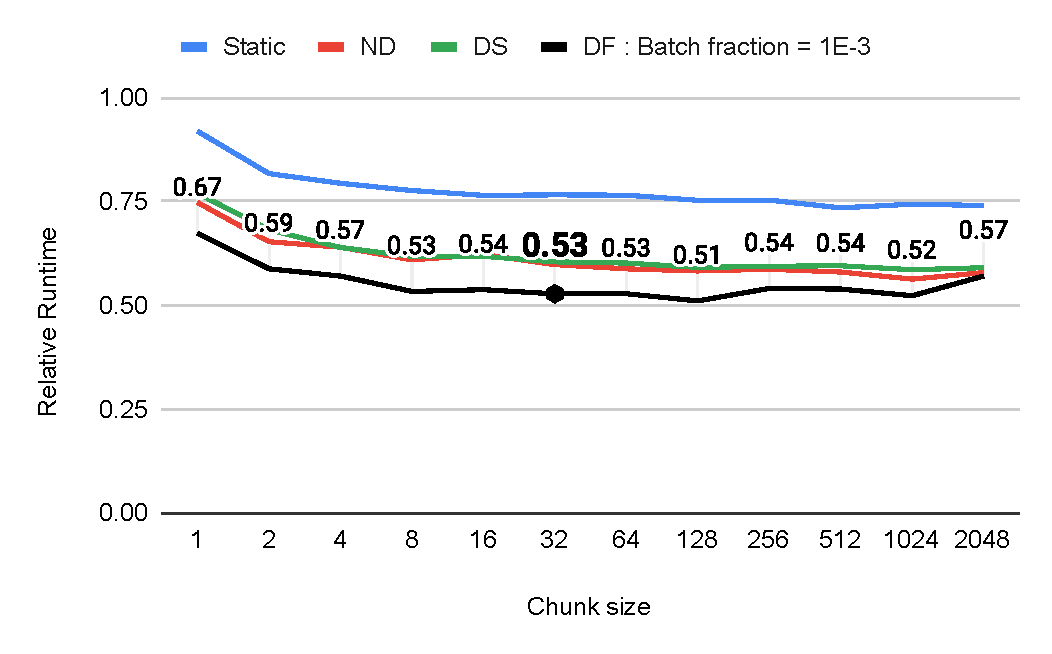
\includegraphics[width=0.98\linewidth]{out/aggregation-adjust-chunksize3.pdf}
  } \\[-1ex]
  \caption{Relative Runtime of \textit{Static}, \textit{Naive-dynamic (ND)}, \textit{Delta-screening (DS)}, and \textit{Dynamic Frontier (DF)} Leiden, with varying dynamic schedule chunk size (OpenMP), for aggregation phase of the Leiden algorithm. These tests were conducted on large graphs, with batch updates randomly generated at sizes of $10^{-7}|E|$, $10^{-5}|E|$, and $10^{-3}|E|$. The results suggest that a chunk size of $32$ is optimal (highlighted).}
  \label{fig:aggregation-adjust-chunksize}
\end{figure}

\begin{figure}[!hbt]
  \centering
  \subfigure{
    \label{fig:subrefine-optimize--8020}
    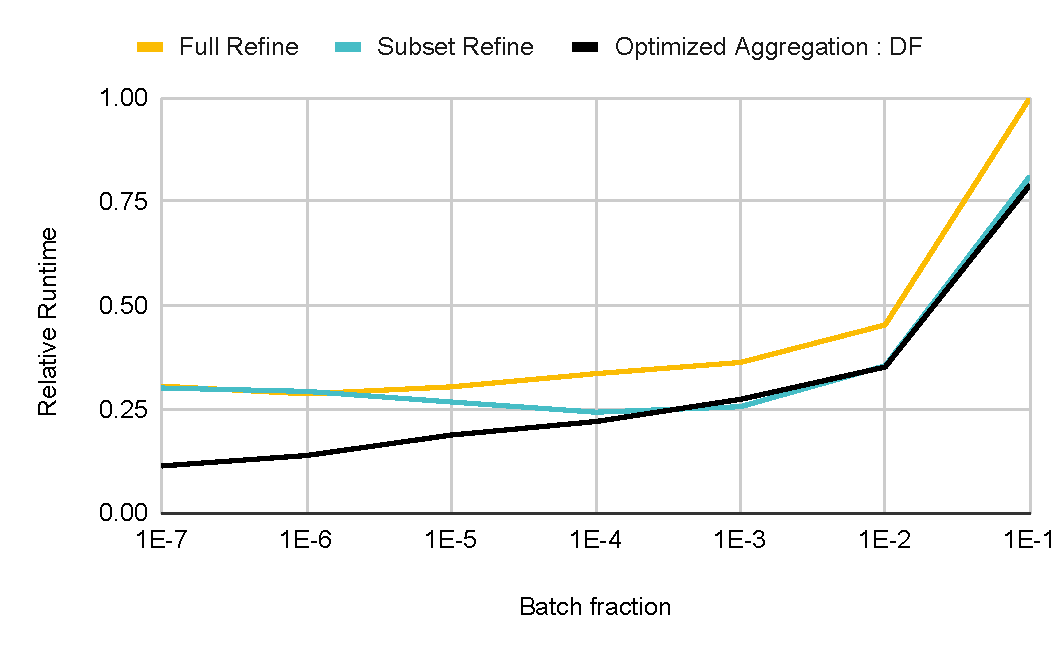
\includegraphics[width=0.98\linewidth]{out/subrefine-optimize-8020.pdf}
  } \\[-2ex]
  \caption{Relative Runtime of \textit{Dynamic Frontier (DF)} approach applied to the Leiden algorithm, incorporating three successive optimizations: \textit{Full Refine}, \textit{Subset Refine}, and \textit{Optimized Aggregation}. These are tested on large graphs with randomly generated batch updates of size $10^{-7}|E|$ to $0.1|E|$, consisting of $80\%$ edge insertions and $20\%$ deletions.}
  \label{fig:subrefine-optimize}
\end{figure}


The pseudocode for \textit{Optimized Aggregation} based ND, DS, and DF Leiden, which we from here on refer to simply as ND, DS, and DF Leiden, respectively, is presented in Algorithms \ref{alg:naive}, \ref{alg:delta}, and \ref{alg:frontier}, with detailed explanations in Sections \ref{sec:our-naive}, \ref{sec:our-delta}, \ref{sec:our-frontier}, respectively. In the first pass of Leiden algorithm, we process the vertices identified as affected by the DS and DF approaches, initializing the community membership of each vertex based on the membership obtained from the previous snapshot of the graph. In the following passes, all super-vertices are marked as affected and processed according to the Leiden algorithm \cite{sahu2024shared}. Similar to DF Louvain \cite{sahu2024dflouvain}, we use the weighted degrees of vertices and the total edge weights of communities as auxiliary information \cite{sahu2024dflouvain}\ignore{, as illustrated in Figure \ref{fig:about-auxiliary}}. Note that guarantees of the original Leiden algorithm \cite{com-traag19} extend to our methods as selective refinement only prunes untouched communities, while processing remaining communities identically to original Leiden.




\subsection{Implementation details}
\label{sec:implementation-details}

We use an asynchronous version of Leiden, where threads independently process different graph parts, enabling faster convergence but increasing variability in the final result. Each thread has its own hashtable to track delta-modularity during the local-moving and refinement phases and the total edge weight between super-vertices in the aggregation phase. Optimizations include OpenMP's dynamic loop schedule, limiting iterations to $20$ per pass, a tolerance drop rate of $10$ starting at $0.01$, vertex pruning, using parallel prefix sums and preallocated Compressed Sparse Row (CSR) data structures for super-vertex graphs and community vertices, and using fast, collision-free per-thread hashtables\ignore{for all algorithm phases} \cite{sahu2024fast}.

For simplicity, we do not skip the aggregation phase of Leiden algorithm, even if a small number of communities are being merged together, unlike the original implementation of Static Leiden \cite{sahu2024fast}. This allows us to maintain a high quality of obtained communities while incurring only a minor increase in runtime across Static, ND, DS, and DF Leiden. Additionally, we employ the refine-based variation of Leiden, where the community labels of super-vertices are determined by the refinement phase rather than the local-moving phase (i.e., move-based)\ignore{\cite{sahu2024fast}}, as the latter would not permit community splits in the scenarios outlined in Section \ref{sec:subset-refine-method}.


\subsection{Time and Space complexity}

The time complexity of ND, DS, and DF Leiden is the same as Static Leiden, i.e., $O(L|E^t|)$, where $L$ is the total number of iterations performed. However, the cost of local-moving and refinement phases in the first pass is reduced, and depends both on the size and nature of the batch update. The space complexity of our algorithms is also the same as Static Leiden, i.e., $O(T|V^t| + |E^t|)$, where $T$ represents the number of threads used ($T|V^t|$ is the space used by per-thread collision-free hashtables \cite{sahu2024fast}).
% \begin{figure}[hbtp]
  \centering
  \subfigure{
    \label{fig:about-auxiliary--with}
    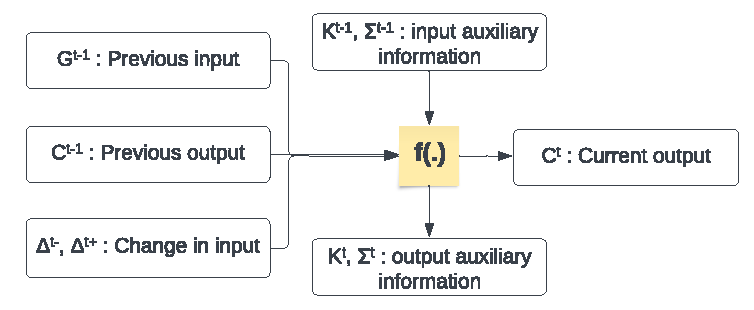
\includegraphics[width=0.98\linewidth]{out/about-auxiliary-with.pdf}
  } \\[-2ex]
  \caption{A dynamic community detection algorithm $f(.)$ takes as input the previous graph $G^{t-1}$, community memberships $C^{t-1}$, and the batch update $\Delta^{t-}$, $\Delta^{t+}$, and produces the updated community memberships $C^t$. However, it may also consider additional information such as the weighted degrees of vertices $K^{t-1}$ and the total edge weights of communities $\Sigma^{t-1}$ as auxiliary information, and yield updated auxiliary information $K^t$, $\Sigma^t$ \cite{sahu2024dflouvain}.}
  \label{fig:about-auxiliary}
\end{figure}

